\section{模型改造与两方安全推理链路}

模型实现遵循“明文训练、密态执行语义重写、双向隐私推理落地”三层结构。训练阶段保留 DynamicViT 的词元打分与样本级动态边界能力；部署阶段将删除式剪枝语义改写为固定图可执行的掩码化表达；推理阶段由 SPU 与 OpenBumbleBee 两方安全推理集成层承担密态执行，仅对外返回最终分类结果。该实现路径的目标不是复现一条完全等价的可变长明文执行图，而是在固定图安全执行约束下尽可能保留动态剪枝边界的判别价值。

对应到动态词元剪枝的核心计算关系，医疗动态安全剪枝链路不再直接删除词元，而是先确定当前 stage 的保留边界，再生成固定形状的 keep-mask，并据此完成后续安全选择。关键关系见式（3-1）至式（3-2e）：

\begin{equation}
\tau^{(l)}=\operatorname{TopKBoundary}\!\left(s^{(l)},K^{(l)}\right), \quad m_i^{(l)}=\mathbf{1}\!\left[\left(s_i^{(l)},i\right)\ge \tau^{(l)}\right]
\tag{3-1}
\end{equation}

\begin{equation}
\tilde{h}_i^{(l)}=m_i^{(l)} \cdot h_i^{(l)}
\tag{3-2}
\end{equation}

\begin{equation}
e_i^{(l)}=s_i^{(l)}-\epsilon \cdot i
\tag{3-2a}
\end{equation}

\begin{equation}
\pi^{(l)}=\operatorname{BitonicSortDesc}\!\left(e^{(l)}\right), \quad m_i^{(l)}=\mathbf{1}\!\left[i\in \pi^{(l)}_{1:K^{(l)}}\right]
\tag{3-2b}
\end{equation}

其中，$s^{(l)}$ 表示第 $l$ 个剪枝 stage 的词元得分向量，$K^{(l)}$ 表示该 stage 允许保留的词元数，$\tau^{(l)}$ 表示由排序边界导出的保留阈值，$e_i^{(l)}$ 表示引入索引微扰后的编码键，$\pi^{(l)}$ 表示经编码键双调排序得到的索引排列，$m_i^{(l)}$ 表示第 $i$ 个词元的保留掩码。报告正文中的安全选择原语 $F_{\text{mux}}$ 与安全比较原语 $F_{\text{less}}$ 正是围绕这组关系完成的协议友好改写。

式（3-2a）与式（3-2b）对应当前密态执行中的并列分数稳定化策略：先通过编码键将词元得分与索引绑定，再在固定比较网络中执行按索引跟踪的双调排序，最后直接从排序结果的前个索引构造 keep-mask。这样做避免了“先排序求阈值、再对全体词元执行一次阈值比较”的二次密态比较开销，同时保证并列分数情况下的保留决策具有确定性。

\begin{equation}
K^{(l)}=\left\lceil \rho^{(l)} N^{(l)} \right\rceil, \quad N_{\text{out}}^{(l)}=\sum_{i=1}^{N^{(l)}} m_i^{(l)}
\tag{3-2c}
\end{equation}

\begin{equation}
b_i^{(l)}=F_{\text{less}}\!\left(\tau^{(l)}, s_i^{(l)}\right)
\tag{3-2d}
\end{equation}

\begin{equation}
\tilde{h}_i^{(l)}=F_{\text{mux}}\!\left(b_i^{(l)}, h_i^{(l)}, 0\right)
\tag{3-2e}
\end{equation}

式（3-2c）进一步给出每个剪枝 stage 的保留预算约束；式（3-2d）与式（3-2e）则分别把保留判定与安全选择写为 $F_{\text{less}}$ 和 $F_{\text{mux}}$ 原语。其中，$\rho^{(l)}$ 表示第 $l$ 个阶段的目标保留率，$N^{(l)}$ 表示该阶段输入词元数，$N_{\text{out}}^{(l)}$ 表示 keep-mask 作用后的实际保留词元数，$b_i^{(l)}$ 表示第 $i$ 个词元在该阶段的安全比较结果。

考虑到本作品的核心创新在于将 DynamicViT 的删除式剪枝重写为固定图下可执行的 keep-mask 语义，算法2进一步给出动态词元剪枝的安全化执行步骤。该算法与式（3-1）至式（3-2e）一一对应，用于说明词元打分、编码排序、保留掩码构造与安全选择之间的实现关系。

图 3-1 从实现结构角度补充展示当前项目框架：上层对应医院终端、业务网关与双节点密态执行域；中层分别对应控制面闭环、DynamicViT 安全化重写组件与两方半诚实安全计算协议；底层则是秘密分享、比较/选择与审计摘要等密码学基础原语。该图用于说明第 2 章“系统设计”与第 3 章“系统实现”的衔接关系。

\begin{figure}[htbp]
\centering
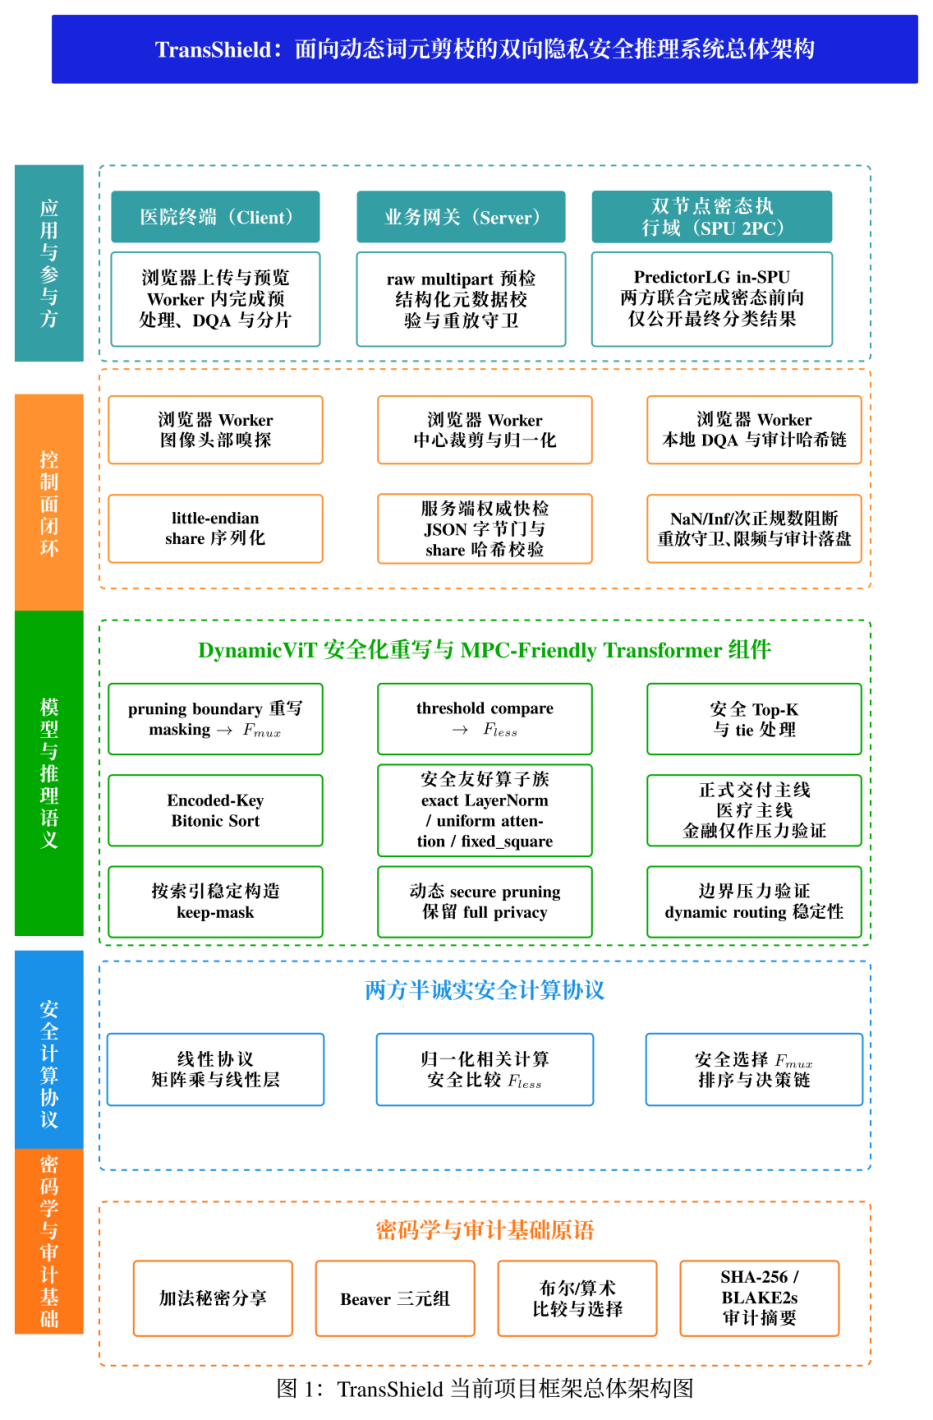
\includegraphics[width=0.92\textwidth]{figures/fig3-1-project-architecture.png}
\caption{图3-1 密捷项目当前框架总体架构图。}
\end{figure}

图3-1可按“终端本地明文处理—跨域密态传输—服务端入口门控—双节点密态执行—结果回传与审计固化”五个层次理解。图左侧的医院终端代表数据提供方，也是整条链路中唯一允许接触原始影像、明文像素张量和局部质量指标的位置；图右侧的双节点密态执行域代表模型持有方与协同计算方在两方半诚实安全计算约束下共同完成推理的区域；两者之间由业务网关和服务端控制面构成一道明确的信任边界。

从输入侧开始，用户在浏览器端选择影像后，主线程并不直接承担高开销计算，而只负责文件句柄保留、界面状态维护与请求编排。真正的图像头部尺寸检查、异常尺寸阻断、解码、中心裁剪、像素归一化、本地数据质量评估、审计哈希链构建以及 share0/share1 的小端序 Float32 序列化，全部在浏览器工作线程内部完成。换言之，图3-1中“医院终端”内部已经同时完成了明文处理、质量预检与秘密分享三项职责，这是原始像素不越出终端侧的关键。

当终端侧形成两份密态分片与结构化元数据后，跨越信任边界传输的对象就被严格限制为：share 字节流、审计摘要和最小必要的结构化质量信息，而不是原始图像或可逆像素值。进入服务端后，业务网关首先负责请求体大小、boundary 参数、多部件结构和字段集合的快速预检；随后，权威快检模块继续完成 JSON 字节长度门、share 哈希校验、内存对齐复制、非有限数与次正规数阻断、张量幅值检查、质量摘要容差复核、nonce 重放拦截、payload 去重以及来源地址并发守卫。只有在这些门控全部通过后，请求才会被转送至下游 SPU 密态执行域。

图3-1中部的 DynamicViT 安全化重写组件用于说明：本作品并不是把一个静态模型简单包进安全计算框架，而是对动态词元剪枝路径本身做了协议友好改写。具体而言，PredictorLG 在 SPU 内部生成词元得分，编码键排序网络在固定图中完成稳定的保留边界推导与 keep-mask 构造，后续 attention、MLP、残差连接和分类头始终保持在两方安全执行域内运行。这样既保留了按样本变化的动态剪枝能力，又避免把剪枝决策暴露为外部明文控制流，从而使“动态”与“密态”真正统一到同一条执行链路中。

在输出侧，SPU 域对外仅释放最终分类结论，而不会泄露中间特征、模型参数或任一方的明文 share。服务端控制面同时补充返回质量裁决、审计摘要与控制面耗时，并将关键事件写入审计记录，以便展示、复核与赛后核查使用同一条证据链。因此，图3-1不仅展示了系统由哪些模块构成，更重要的是交代了每一类数据在什么位置生成、在什么边界停止、由谁执行校验，以及最终以何种最小暴露形式返回结果；沿着这条责任链阅读，即可完整理解本作品从上传、门控、推理到审计的整体运作流程。

与固定结构 Transformer 私有推理路线相比，本作品在模型改造阶段优先解决的是“动态决策链如何留在安全执行域内”。Iron[18]、BOLT[19]、BumbleBee[7] 和 NEXUS[20] 主要围绕固定结构模型的矩阵乘、Softmax、LayerNorm、GELU 或交互轮次进行协议级优化；而本作品首先保留视觉 DynamicViT 的逐 stage 保留语义，再把删除式剪枝重写为 keep-mask 驱动的固定图执行。这一差异决定了本作品的贡献重点不在于单独压缩某个算子，而在于让动态词元剪枝本身能够在两方安全执行链路中稳定落地。

\section{端到端执行流程与模块协同}

结合图 3-1 的当前项目框架，当前端到端链路可以压缩为三个安全阶段。第一阶段是终端本地预处理：浏览器工作线程完成影像解码、质量评估、审计链构建与秘密分享，安全目标是使原始影像和明文像素止于终端侧。第二阶段是服务端边界拦截：前置网关与权威快检模块在进入 SPU 之前完成报文、结构化元数据、share 字节流与重构张量合法性校验，安全目标是使异常输入、重放请求和畸形张量止于密态执行入口之外。第三阶段是 SPU 密态执行：PredictorLG、编码键排序、keep-mask 构造与前向分类全部保留在两方安全执行域内，安全目标是避免动态决策链退化为外部明文回放。

因此，本节不再重复图 2-2 中的逐步动作，而是强调各阶段的安全职责分工：前端负责明文边界与分片生成，服务端负责权威阻断与审计固化，SPU 路径负责完成双向隐私约束下的动态安全推理。

\section{前端控制面实现}

前端实现采用主线程与单实例浏览器工作线程分离的结构。主线程只负责文件句柄保留、页面状态维护和请求编排；工作线程内部完成图像头部尺寸嗅探、异常尺寸阻断、解码与中心裁剪、数据质量指标提取、源图与 share 审计哈希计算、小端序 32 位浮点（Float32）字节流序列化与可转移数组缓冲区传递。该设计避免了大体量数组在主线程上的结构化克隆开销，同时将高开销计算与页面交互解耦。

前端计算过程中的关键数值变换、两方分片关系与审计关系见式（3-3）至式（3-5），其中式（3-4a）进一步给出输入张量与两方 share 之间的对应关系：

\begin{equation}
x_{c,h,w}=\operatorname{clip}\!\left(\frac{\frac{p_{c,h,w}}{255}-\mu_c}{\sigma_c},-2,2\right)
\tag{3-3}
\end{equation}

\begin{equation}
\operatorname{share0}_{c,h,w}=r_{c,h,w}, \quad r_{c,h,w}\sim U[-2,2], \quad \operatorname{share1}_{c,h,w}=x_{c,h,w}-\operatorname{share0}_{c,h,w}
\tag{3-4}
\end{equation}

\begin{equation}
x_{c,h,w}=\langle x_{c,h,w}\rangle_{0}+\langle x_{c,h,w}\rangle_{1}, \quad \langle x_{c,h,w}\rangle_{0}=\operatorname{share0}_{c,h,w}, \quad \langle x_{c,h,w}\rangle_{1}=\operatorname{share1}_{c,h,w}
\tag{3-4a}
\end{equation}

\begin{equation}
H_{\text{audit}}=\operatorname{SHA256}\!\left(v7 \parallel nonce \parallel H(src) \parallel H(x) \parallel H(\operatorname{share0}) \parallel H(\operatorname{share1})\right)
\tag{3-5}
\end{equation}

其中，$p_{c,h,w}$ 表示裁剪后图像在通道 $c$、位置 $(h,w)$ 的原始像素值，$\mu_c$ 与 $\sigma_c$ 分别对应 ImageNet 均值与标准差，$x_{c,h,w}$ 为送入模型的归一化张量值；式（3-4a）中的 $\langle x_{c,h,w}\rangle_0$ 与 $\langle x_{c,h,w}\rangle_1$ 对应浏览器端生成的两份 additively split share，并在传输层分别落到 share0 与 share1。为避免浏览器端异常数值写入底层缓冲区，前端会先将归一化结果裁剪到 [-2, 2]，再以 little-endian Float32 方式写入 share 字节流；审计链则把源图哈希、归一化张量哈希与两份 share 哈希绑定到同一个 nonce 上。

为便于直观看清主线程与浏览器工作线程的职责边界，图 3-2 将文件句柄保留、页面状态维护、可转移数组缓冲区传递、图像预处理、审计哈希与秘密分享生成拆解为三个协同区域。该图对应本节实现要点：主线程只负责交互与调度，工作线程承担高开销计算，并在跨越信任边界前完成明文终止与密态分片生成。

\begin{figure}[htbp]
\centering
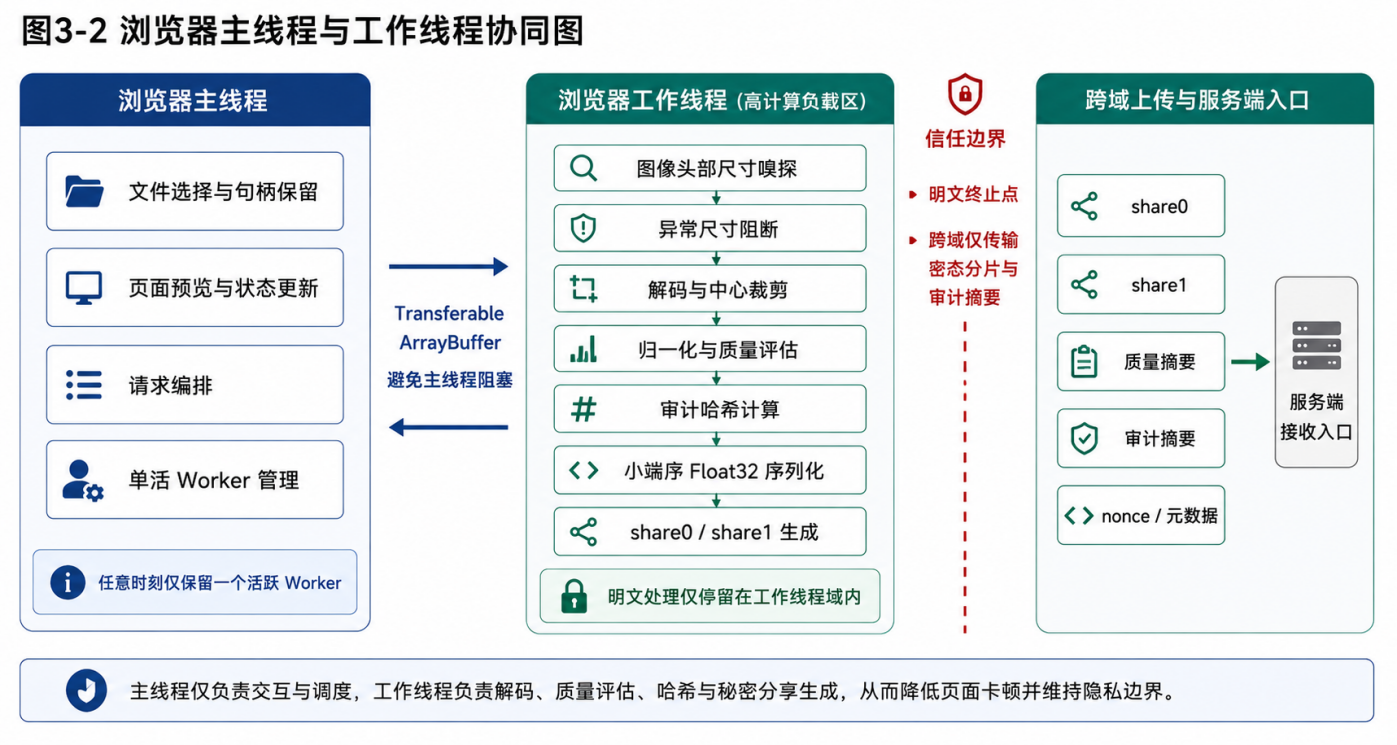
\includegraphics[width=0.92\textwidth]{figures/fig3-2-browser-worker-collaboration.png}
\caption{图3-2 浏览器主线程与工作线程协同图：主线程负责交互与调度，工作线程负责预处理、哈希与秘密分享生成。}
\end{figure}

\section{服务端权威快检与审计}

服务端在进入 SPU 之前，依次执行原始报文体读取上限、boundary 参数解析、多部件表单（multipart）原始结构预检、精确字段集约束、单字段 JSON 字节长度门、严格 UTF-8 结构化元数据解析、share 哈希校验、张量重构前内存对齐复制、非有限数与次正规数阻断、服务端数据质量复核，以及 nonce、payload 与来源 IP 维度的重放与并发守卫。审计层同时记录哈希摘要、控制面开销与事件落盘结果，以保证前端展示、服务端阻断与事后核查使用的是同一条证据链。

服务端快检并非只核对客户端声明，而是围绕重构张量、质量摘要与容差关系进行权威复算。关键关系见式（3-6）至式（3-9b），其中式（3-6a）给出最终分类输出的恢复关系：

\begin{equation}
X=\operatorname{share0}+\operatorname{share1}, \quad RGB=X\odot \sigma+\mu
\tag{3-6}
\end{equation}

\begin{equation}
z_c=\langle z_c\rangle_{0}+\langle z_c\rangle_{1}, \quad \hat{y}=\arg\max_c z_c
\tag{3-6a}
\end{equation}

\begin{equation}
L_i=0.299R_i+0.587G_i+0.114B_i, \quad \operatorname{OverExp}=\frac{1}{N}\sum_{i=1}^{N}\mathbf{1}\!\left[L_i\ge 0.95\right]
\tag{3-7}
\end{equation}

\begin{equation}
\operatorname{lap}(x,y)= -4L(x,y)+L(x-1,y)+L(x+1,y)+L(x,y-1)+L(x,y+1)
\tag{3-8}
\end{equation}

\begin{equation}
\Delta_k=\left|q_k^{(\text{client})}-q_k^{(\text{server})}\right|, \quad \Delta_k \le 10^{-4}
\tag{3-9}
\end{equation}

\begin{equation}
\mu_{\text{lap}}=\frac{1}{HW}\sum_{x=1}^{H}\sum_{y=1}^{W}\operatorname{lap}(x,y), \quad \sigma_{\text{lap}}^{2}=\frac{1}{HW}\sum_{x=1}^{H}\sum_{y=1}^{W}\left(\operatorname{lap}(x,y)-\mu_{\text{lap}}\right)^{2}
\tag{3-8a}
\end{equation}

\begin{equation}
F_{\text{payload}}=\operatorname{BLAKE2s}\!\left(H(\operatorname{share0}) \parallel \text{:} \parallel H(\operatorname{share1})\right)
\tag{3-9a}
\end{equation}

\begin{equation}
n_{\text{ip}}(t;\Delta)=\sum_j \mathbf{1}\!\left[t-\Delta \le t_j \le t\right], \quad n_{\text{ip}}(t;\Delta)\le R_{\text{ip}}, \quad c_{\text{ip}}^{\text{inflight}}\le C_{\text{ip}}
\tag{3-9b}
\end{equation}

式（3-6a）给出最终类别 logit 的两方恢复关系；式（3-8a）将离散拉普拉斯响应进一步归约为方差指标，用于度量局部纹理与边缘强度；式（3-9a）与式（3-9b）分别对应载荷指纹去重与来源地址限频 / 并发守卫，从而把服务端控制面中的“去重、限频、准入”逻辑形式化为可验证约束。

其中，服务端会先对 share 执行内存对齐复制，再将绝对值小于 $2^{-126}$ 的极小值刷新为零，以切断次正规数带来的微代码异常路径；随后检查 share 与重构张量是否存在非有限值，以及 share 幅值是否超过 $2$。对客户端与服务端分别得到的质量摘要 $q_k^{(\text{client})}$ 与 $q_k^{(\text{server})}$，只在基础连续数值出现显著偏离时才标记可疑漂移，而不会仅凭离散风险标签不一致就直接判定篡改。

为了把服务端权威快检、重放防护、并发守卫与审计落盘过程概括为可执行步骤，算法3给出服务器侧的统一验证与审计流程。

为便于对应服务端控制面的实际落地点，图 3-3 将权威快检与审计闭环拆解为原始请求体读取、协议结构预检、JSON 长度门、share 哈希校验、张量快检、重放并发守卫与审计落盘等连续门控步骤。该图与本节公式部分共同说明：客户端声明不会直接成为最终裁决依据，请求只有在全部检查通过后才会进入 SPU 密态执行域。

本章出现的核心数学符号及其含义汇总如表 5 所示。

\begin{figure}[htbp]
\centering
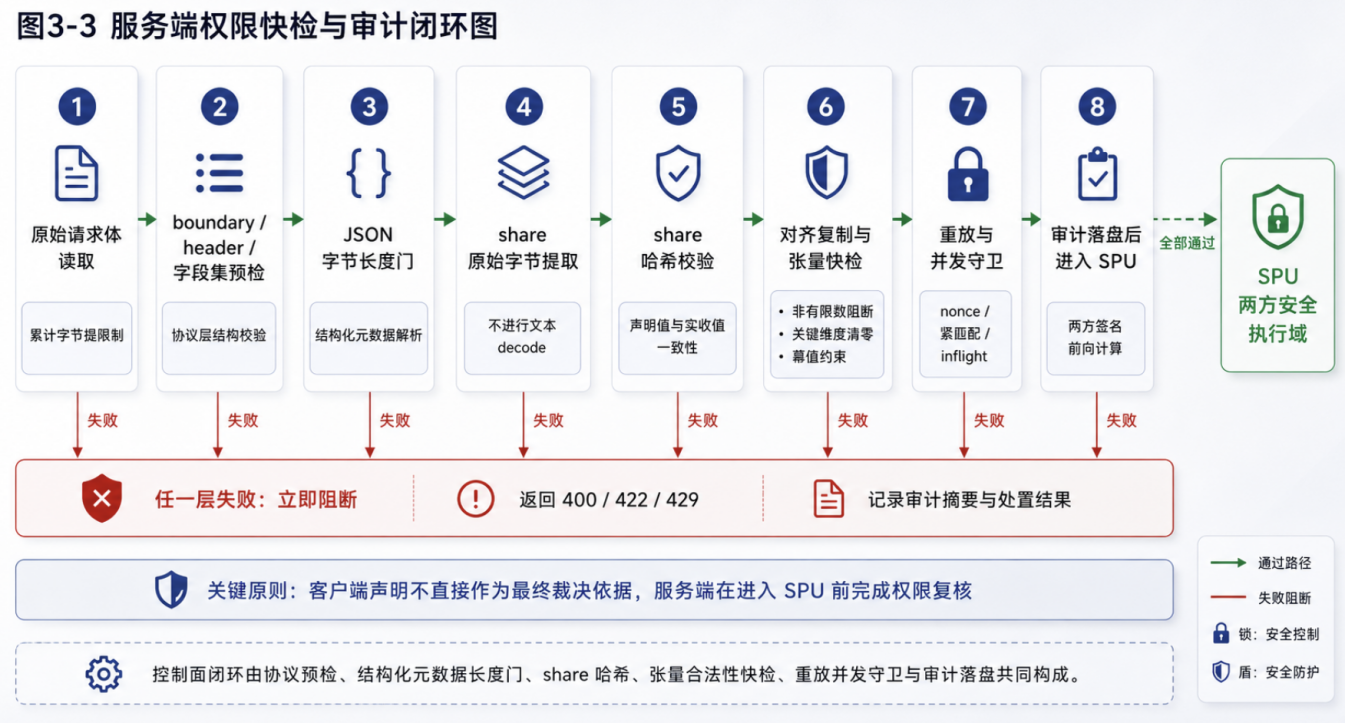
\includegraphics[width=0.92\textwidth]{figures/fig3-3-control-plane-gates.jpeg}
\caption{图3-3 服务端权威快检与审计闭环图：请求仅在全部门控通过后进入 SPU，任一层失败均立即阻断并记录审计结果。}
\end{figure}

\begin{longtable}{>{\raggedright\arraybackslash}p{0.32\textwidth}>{\raggedright\arraybackslash}p{0.32\textwidth}>{\raggedright\arraybackslash}p{0.32\textwidth}}
\caption{表 5 第三章关键符号说明}\\
\toprule
\textbf{符号} & \textbf{含义} & \textbf{出现位置} \\
\midrule
\endfirsthead
\toprule
\textbf{符号} & \textbf{含义} & \textbf{出现位置} \\
\midrule
\endhead
 & 第 l 个剪枝 stage 的词元得分向量 & 式(3-1) \\
 & 第 l 个剪枝 stage 允许保留的词元数 & 式(3-1) \\
 & 由安全 Top-边界导出的保留阈值 & 式(3-1) \\
 & 编码键与经双调排序得到的索引排列 & 式(3-2a)、式(3-2b) \\
 & 第 i 个词元在第 l 个 stage 的保留掩码 & 式(3-1)、式(3-2)、式(3-2b) \\
 & 原始词元表征与掩码后的词元表征 & 式(3-2) \\
 & 裁剪后图像在通道 c、位置 (h,w) 的原始像素值 & 式(3-3) \\
 & 通道 c 的归一化均值与标准差 & 式(3-3)、式(3-6) \\
 & 归一化后的模型输入张量 & 式(3-3)、式(3-4) \\
 & 针对输入张量构造的两份秘密分享分片 & 式(3-4) \\
 & 第 k 个质量指标及其客户端/服务端绝对偏差 & 式(3-9) \\
 & 像素总数、亮度值与离散拉普拉斯响应 & 式(3-7)、式(3-8) \\
\bottomrule
\end{longtable}

\section{关键交付物与证据落点}

本作品的核心交付物、仓内存储路径与用途说明如表 6 所示。

工程实现上，模型部署包不仅包含权重和推理参数，还包含用于解释执行边界的 manifest 信息。该信息用于约束输入形状、剪枝阶段、保留比例、近似算子配置和审计字段，使训练导出的模型语义、SPU 执行闭包和前端展示内容能够相互校验。这样做可以降低“模型已更新但展示仍引用旧指标”或“配置变更后安全边界描述失真”的风险，也使报告中的实验指标能够回溯到仓内实际文件。

\begin{longtable}{>{\raggedright\arraybackslash}p{0.32\textwidth}>{\raggedright\arraybackslash}p{0.32\textwidth}>{\raggedright\arraybackslash}p{0.32\textwidth}}
\caption{表 6 系统关键交付物与仓内落点说明}\\
\toprule
\textbf{类别} & \textbf{仓内落点} & \textbf{用途} \\
\midrule
\endfirsthead
\toprule
\textbf{类别} & \textbf{仓内落点} & \textbf{用途} \\
\midrule
\endhead
前后端演示程序 & showcase/src/；showcase/src/workers/medicalControlPlaneWorker.ts；showcase\_api/app.py；showcase\_api/control\_plane.py & 承载浏览器工作线程、服务端权威快检、页面交互与 /api/medical/live-run 入口 \\
自动化验证脚本 & tools/showcase\_protocol\_fuzz.py；tools/showcase\_guard\_stress.py & 验证协议层异常输入、重放与并发守卫 \\
图件与报告生成脚本 & tools/showcase\_extract\_report\_assets.py；showcase/public/report-assets/；showcase/src/generated/report\_content.json & 从正式 DOCX 提取展示图件与章节 JSON，用于重建展示站内容 \\
复现说明 & README\_REPRODUCE.md & 提供环境约束、运行步骤与预期输出 \\
许可证与修改映射 & spu\_vendored/LICENSE；spu\_vendored/MODIFICATIONS.md；THIRD\_PARTY.md & 支撑第三方许可与本地修改说明 \\
\bottomrule
\end{longtable}

\noindent\textit{注：所有交付物均已纳入版本控制，仓内路径与本表格完全一致；自动化验证脚本可直接运行生成对应证据文件。}
